\section{Embedding}\label{chap:embedding}
        
    \paragraph{}Our next objective centers on the conversion of raw byte data into fixed-size embeddings (\ref{seq:background:traditional_statistical_embedding}, \ref{seq:background:deep_learning_models_for_raw_byte_embedding}), a pivotal step in preparing them for utilization in machine learning applications. Ensuring uniformity in embedding size across all memory structures holds paramount significance. Consistency in embedding dimensions is vital to empower machine learning algorithms for efficient data processing and analysis. This uniformity not only simplifies the integration of memory structures with varying sizes into a coherent classification framework but also acts as a defense against the adverse effects of the curse of dimensionality—a phenomenon that can introduce computational complexities and heighten the risk of overfitting in high-dimensional data spaces. Striking this equilibrium is essential, achieved by maintaining reasonably low embedding dimensions, fostering both efficient data processing and the preservation of essential information within the raw byte data. It's important to note that initially, each embedding will include the structure's file and the structure's address in the file. However, these details will be removed during the machine learning phase (quality or coherence) as the embedding aims to be free of key size or OpenSSH uses. Their presence will serve as a means to test coherence later in our analysis.

\subsection{First Preprocessing}
    \paragraph{}Initially, we possess some knowledge regarding the positions and characteristics of SSH keys. Leveraging this knowledge, we can narrow down the number of chunks to examine, thereby streamlining the analysis process.
    
    \subsubsection{Entropy-Based Approach}
        \paragraph{}A distinctive feature of SSH keys is their inherent randomness, as referenced in section \ref{seq:background:traditional_statistical_embedding}. This randomness translates to a high entropy value for the keys. By focusing on chunks with high entropy, we can potentially isolate those that contain SSH keys.
        
        \paragraph{}To compute the entropy, we consider the minimal size of a key, which is 12 bytes as mentioned in section \ref{sec:methods:keys_analysis}. Given that a chunk has a minimum of 2 blocks, equivalent to 16 bytes as detailed in section \ref{sec:background:dataset:c_structures_and_chunks_allocation_understanding}, and the fact that keys are always positioned at the beginning of a chunk, we can extract the first 12 bytes of a chunk to compute its entropy.
        
        \paragraph{}Given the abundance of data at our disposal, it's feasible to focus solely on chunks with the highest entropy values. However, it's crucial to remember that this is a heuristic approach. There's a need to be vigilant and ensure that important nodes with slightly lower entropy, possibly due to random occurrences like two identical bytes in the initial 12 bytes, are not inadvertently excluded from the analysis. Due to the potential risk of missing out on some keys with this filter, it is advisable to apply it only during the training phase and not in the validation phase. However, for the sake of simplicity in our approach, we will apply this filter in the validation phase as well, taking extra care to add any missing keys back into the dataset to ensure completeness and accuracy in our analysis.
    \subsubsection{Chunk Size Filter}
        \paragraph{}Our analysis of SSH key chunks has shown that they are always either 32, 48, or 64 bytes in size. This observation allows us to apply a filter based on chunk size, selecting only chunks of these specific sizes for further analysis and discarding the rest. This method of selection helps to streamline the analysis process and ensures that we are focusing on the most relevant chunks.
        
        \paragraph{}By combining the entropy-based approach and the chunk size filter, we can avoid the need for random subsampling. This is particularly advantageous as our dataset is not significantly imbalanced, provided that these filters are applied.
    

\subsection{Basic Chunk Information}\label{seq:embedding:basic_chunk_information}

    \paragraph{}Every chunk in the heap dump is equipped with a set of fundamental details that provide insights into its structure and content. These basic pieces of information are essential for understanding the layout and composition of each chunk.

    \paragraph{}It's important to note that these foundational details are not exclusive to just the primary chunk nodes. Value nodes and pointer nodes, which might be considered as sub-components of a chunk, also inherit these basic attributes from their parent chunk node.

    \paragraph{}The core information associated with each chunk includes:

    \begin{itemize}
        \item \textbf{block\_position\_in\_chunk}: This represents the position of a specific block within the chunk. For the primary chunk node, this value is always 0, indicating the start of the chunk.
        
        \item \textbf{chunk\_byte\_size}: This provides the total size of the chunk, measured in bytes.
        
        \item \textbf{chunk\_ptrs}: This denotes the total number of pointers present within the chunk.
        
        \item \textbf{chunk\_vns}: This indicates the total number of value nodes contained within the chunk.
        
        \item \textbf{chunk\_number\_in\_heap}: This value represents the index or position of the chunk within the entire heap, giving a relative placement of the chunk in the context of all chunks.
    \end{itemize}

    With these basic details, one can gain a comprehensive understanding of each chunk's structure, content, and relative position within the heap.

\subsection{Statistical embedding}\label{sec:embedding:statistical}
    \paragraph{}Understanding the fundamental concepts of statistical embeddings enables us to delve deeper into the sophisticated processes and practical applications that underscore their significance in embedding tasks. By utilizing statistical techniques, data from high-dimensional spaces is condensed, preserving the inherent probabilistic connections and essential patterns as much as possible.

    \subsubsection{N-gram values}
        \paragraph{}In reference to section \ref{seq:background:byte_frequency_distribution}, we adopt the use of n-gram values, specifically focusing on the frequency of byte combinations. However, an implication of this approach is that it leads to an exponentially high dimensional space. For instance, with a 2-gram, the potential values amount to $256*256=65536$. Given the extensive dimensionality, we have opted for combinations of bits rather than bytes. This change substantially reduces the space required; a 2-gram, in this case, would only amount to $2*2=4$ values.

        \paragraph{}Switching to bit combinations aligns well with our objectives. Our main interest is in the frequency patterns of n-gram values rather than the specific n-gram values themselves. This is because our core aim is to identify SSH keys, which inherently display frequencies for all combinations due to their random nature.

        \paragraph{}In our approach, we utilize 1-gram, 2-gram, 3-gram, and 8-gram values (of bits). The inclusion of 8-gram is particularly significant as it captures larger sequences, providing a broader context and enhancing the ability to discern patterns and anomalies that shorter n-grams might miss. Specifically, the 8-gram contributes 256 values to the embedding vector. When combined with the 8 values from the 3-gram, 4 from the 2-gram, and 2 from the 1-gram, the total dimensionality for the n-gram embedding becomes 270. This comprehensive approach ensures a more robust representation of the data, aiding in the accurate identification of SSH keys. Importantly, by opting for an 8-gram, we avoid the exponential growth in dimensionality that a larger n-gram, such as a 16-gram, would introduce, ensuring that the embedding vector remains manageable and doesn't explode in size or in memory usage.
        

    \subsubsection{Other statisticals values}
        \paragraph{}In our approach, several metrics are employed to analyze the data. Specifically, we utilize the mean as detailed in \ref{eq:mean_byte_value}, the standard deviation as found in \ref{eq:standard_deviation}, the MAD from \ref{eq:mad}, the skewness as outlined in \ref{eq:skewness}, the kurtosis referenced in \ref{eq:kurtosis}, and the Shannon entropy from \ref{eq:shannon_entropy}. These metrics, when collectively considered, provide a comprehensive understanding and embed a plethora of information about the data at hand.

        \paragraph{}It's imperative to note a particular aspect of our analysis concerning the standard deviation. There are instances where the standard deviation registers a value of zero. Such an occurrence is indicative of data consistency. Concurrently, in such scenarios, both the kurtosis and skewness are undefined. When faced with this situation, our course of action is to dismiss the \gls{chunk} from our analysis. The rationale behind this is straightforward: a consistent \gls{chunk} would likely not be pertinent to our exploration, especially when our aim is to identify patterns characteristic of an SSH key, wich are random by nature.
    \subsubsection{Statistical Embedding}

        \paragraph{}For each \gls{chunk}, we construct vectors using a combination of n-gram values and other statistical metrics. The n-gram approach contributes 270 distinct values to the vector. Simultaneously, the supplementary statistical metrics, which encapsulate measures of the mean, standard deviation, MAD, skewness, kurtosis, and Shannon entropy, introduce an additional 6 values. Furthermore, as discussed in a preceding section~\ref{seq:embedding:basic_chunk_information}, the basic information associated with each chunk is also embedded into this vector. Consequently, the resultant vector for each structure comprises a total of 281 values, providing a comprehensive representation of the chunk's characteristics.
    
    

\subsection{Graph embedding}\label{sec:embedding:graph_embedding}
    \paragraph{}In this section, we shift our focus towards the creation and embedding of graphs derived from the heap dump data. The process of graph creation involves structuring the data in a way that captures the relationships and connections between the \glspl{chunk} and their \glspl{pointer}. Subsequently, we will transform this graphs into low-dimensional vector representations, enabling the application of machine learning techniques to identifying \glspl{chunk} containing ssh keys.

    \subsubsection{Graphs creation}
        \paragraph{}Our graph construction is a meticulously organized process aimed at representing the intricate relationships present within the heap dump data. Comprising three distinct node types - \glspl{chunk}, \glspl{pointer}, and \glspl{value_node} - this graph provides a comprehensive view of the data's structure. Our approach commences with the sequential parsing of the heap dump data, enabling the identification of essential \glspl{chunk} central to our analytical objectives. These \glspl{chunk} form the core nodes of our graph. To establish connections between these \glspl{chunk} and the data they contain, we further divide each structure into 8-byte blocks, which is the size of the heap alignment. These blocks are then translated into \glspl{value_node} within the graph, serving as connectors bridging the data structures to their specific data. An heuristic approach, grounded in \acrshort{regex}~\ref{seq:methods:dataset:pointer}, is employed to identify valid \glspl{pointer} within the heap dump data, with \glspl{pointer} representing a subset of \glspl{value_node}, indicating legitimate \glspl{pointer} references. The scrupulously established connections between \glspl{chunk}, \glspl{value_node}, and \glspl{pointer} ensure that the graph accurately mirrors the intricate relationships found within the heap dump data. This comprehensive graph construction process is efficiently implemented in Rust, making effective use of the Petgraph library to handle the complexities of heap dump data and graph representation, offering superior efficiency compared to a Python-based implementation.

        \paragraph{}In the following image \ref{fig:graph_embedding:graph_creation_process}, we can see the \glspl{chunk} nodes representing in blue, containing \glspl{pointer} nodes in orange and \glspl{value_node} nodes in gray. 

        \begin{figure}[H]
            \centering
            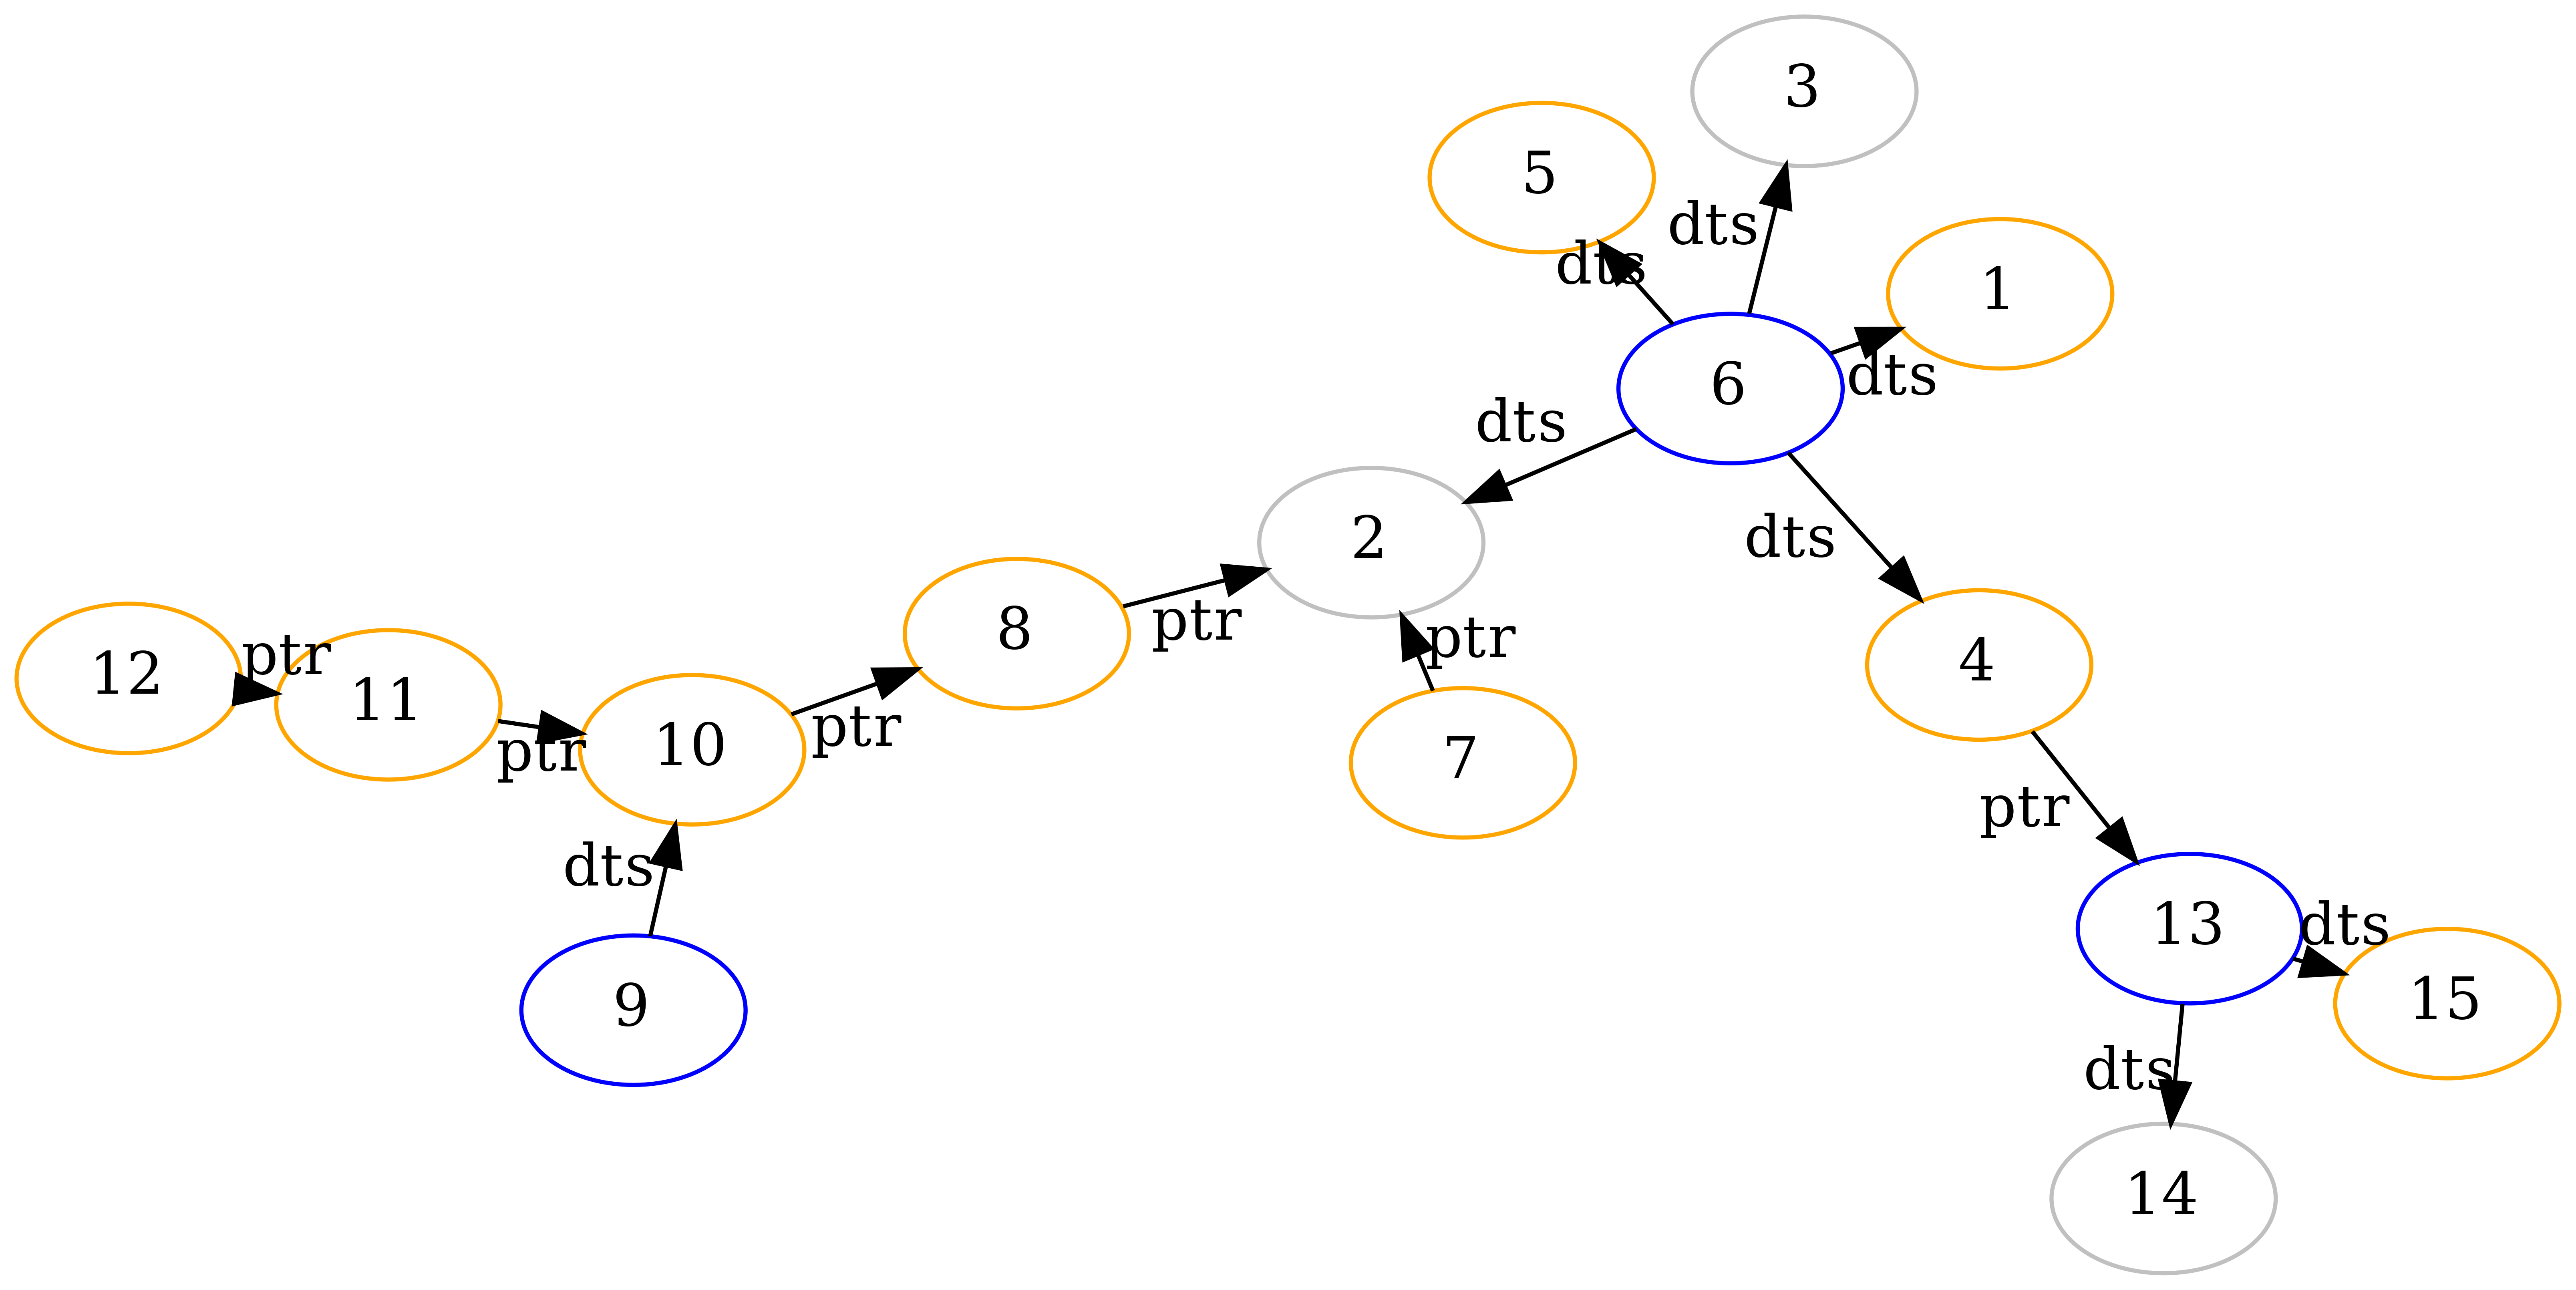
\includegraphics[width=0.9\textwidth]{img/graph_embeding/graph_explain.png}
            \caption{Graph creation process}
            \label{fig:graph_embedding:graph_creation_process}
        \end{figure}

        \paragraph{}After the construction of the graph, we can use graphviz (and the DOT language)\cite{farin_graphviz_2004} to visualize the graph, using the command :
        \begin{lstlisting}[language=bash]
            sfdp -Gsize=67! -Goverlap=prism -Tpng dot_file > image.png
        \end{lstlisting}

        \paragraph{}The following image is an example of the creation of the graph from the file \path{./Validation/Validation/basic/V_8_1_P1/24/27107-1643980590-heap.raw} without \glspl{value_node} to enhance clarity.
        \begin{figure}[H]
            \centering
            \includegraphics[width=0.9\textwidth]{img/graph_embeding/chunk_data_clean_27107-1643980590-heap.raw_dot_no_vn-sfdp.png}
            \caption{Graph example}
            \label{fig:graph_embedding:graph_example}
        \end{figure}

    \subsubsection{Graphs embedding} \label{sec:embedding:first_graph}

        \paragraph{}Our next step is to uncover deeper insights and semantic understanding from our constructed graph, focusing on semantic embedding. This is the process through which we reshape our graph into a low-dimensional vector space, with each vector acting as a repository for a \gls{chunk}'s immediate neighborhood. Through this transformative journey, our aim is to forge vector representations that empower the application of cutting-edge machine learning techniques.

        \paragraph{}To create a concise yet informative representation, considering both structure-to-member and pointer-based connections, we meticulously count the number of \glspl{pointer} and \glspl{chunk} directly referencing a specific \gls{chunk}'s members. This initial count provides valuable insights into the \gls{chunk}'s immediate context. However, we doesn't stop there; we expand this representation by including counts of \glspl{pointer} and \glspl{chunk} pointing to those preceding nodes, allowing us to capture deeper layers of context. This recursive process continues until we reach a predetermined depth. Furthermore, we initiate a parallel analysis in reverse, meticulously tracing connections by following \glspl{pointer} from the initial \gls{chunk} to capture its children, recursively delving deeper until we reach the specified depth. We can see the algorithm here \ref{algo:embedding:generate_ancestor_children_embedding}. The result is a low-dimensional vector that intricately encodes the \gls{chunk}'s neighborhood, offering a comprehensive view of its relationships and contextual significance within the graph.

        \begin{algorithm}[H]
            \caption{Generate Ancestor/Children Embedding}
            \label{algo:embedding:generate_ancestor_children_embedding}
            \begin{algorithmic}
                \Function{GenerateNeighborsCHN}{$chunk\_node, dir$}
                    \State $ancestor\_nodes \gets$ an empty set
                    \State $children \gets$ graph.neighbors\_directed($chunk\_node, OUT$) \Comment{Get members of the chunk}
                    \For{$child$ \textbf{in} $children$}
                        \State $ancestor\_nodes$.insert($child$)
                    \EndFor
                    \State $result \gets$ an empty list
                    \State $current\_nodes \gets$ an empty set
                    \For{$\_$ \textbf{in} $0$ \textbf{to} $DEPTH$}
                        \State $current\_nodes \gets$ $ancestor\_nodes$ \Comment{switch ancestor nodes and current nodes}
                        \State $ancestor\_nodes \gets$ an empty set
                        \State $nb\_chn \gets 0$
                        \State $nb\_ptr \gets 0$
                        \For{$current\_node$ \textbf{in} $current\_nodes$}
                            \If{$node$ is ChunkHeaderNode} \Comment{Update number of chunks and pointers}
                                \State $nb\_chn \gets nb\_dtn + 1$
                            \ElsIf{$node$ is PointerNode}
                                \State $nb\_ptr \gets nb\_ptr + 1$
                            \EndIf
                            \Comment{Get neighbors of the current node}
                            \For{$neighbor$ \textbf{in} graph.neighbors\_directed($current\_node, dir$)}
                                \State $ancestor\_nodes$.insert($neighbor$) \Comment{Add neighbors to the next ancestor nodes}
                            \EndFor
                        \EndFor
                        \State $result$.append($nb\_chn$) \Comment{Add number of data structures}
                        \State $result$.append($nb\_ptr$) \Comment{Add number of pointers}
                    \EndFor
                    \State \textbf{return} $result$
                \EndFunction
            \end{algorithmic}
        \end{algorithm}
        
        \paragraph{}We can apply this algorithm to every \gls{chunk} within each graph, delving to a depth of 8, which produces an embedding of 32 units: 8 for ancestor \glspl{pointer}, 8 for ancestor \glspl{chunk}, 8 for child \glspl{pointer}, and 8 for child \glspl{chunk}. To accurately represent the \gls{chunk}'s neighborhood, it's crucial not to omit details about its members. Thus, we incorporate the basic chunk information, which includes the block position in the chunk, chunk byte size, number of pointers in the chunk, number of value nodes in the chunk, and the chunk's index in the heap. This results in a final embedding size that is an aggregate of the neighborhood representation and the basic chunk information, summing up to 37 values. However, there are inherent challenges with this embedding. It tends to get polluted by the value node, which often lacks significant meaning. Moreover, the relationships between the structures are intricate, and there's potential to represent them in a more straightforward manner, as shown in the next section.

        \paragraph{}\label{sec:embedding:first_graph_only_first_block}To enhance the quality of our embedding, we can introduce an additional layer of refinement: by retaining only the first block of each chunk, we effectively filter out noise nodes. This is based on the knowledge that keys are invariably located at the beginning of a chunk, allowing us to streamline our focus and reduce extraneous data.

    \subsubsection{Updated graph}\label{sec:embedding:updated_graph}

        \paragraph{}Recognizing these challenges and the need for a clearer representation, we embarked on a series of refinements. Our approach focuses on enhancing the last graph by preserving the structure nodes and their interconnections via \glspl{pointer}. To simplify the visualization, we've decided to eliminate both the value nodes and the \gls{pointer} nodes. In addition, the relationships that previously connected the \gls{pointer} nodes to the value nodes will now link directly to the \gls{chunk} nodes, with the added detail of weighted edges. This strategy is driven by our aspiration to offer a more lucid graph, significantly reducing any extraneous noise, as show in the figure \ref{fig:graph_embedding:updated_graph}, the representation of the same file \path{./Validation/Validation/basic/V_8_1_P1/24/27107-1643980590-heap.raw}.

        \begin{figure}[H]
            \centering
            \includegraphics[width=0.9\textwidth]{img/graph_embeding/updated_graph_27107-1643980590-heap.raw_dot_no_vn_chn_annotation_no_vn-sfdp.png}
            \caption{Updated graph}
            \label{fig:graph_embedding:updated_graph}
        \end{figure}

        \paragraph{}By eliminating the pointer nodes, we have successfully integrated their information directly into the relationships between chunk nodes. The embedding now includes 8 preceding depth chunk nodes, 8 subsequent depth chunk nodes, and 5 basic information values, as outlined in section \ref{seq:embedding:basic_chunk_information}. This consolidation results in a compact representation of 21 values, enhancing the embedding's simplicity and efficiency. Although the graph now communicates information more effectively, the embedding has become less detailed. This change in richness could potentially impact the performance of machine learning tasks.

    \subsubsection{Other Graph Embedding Techniques}
        \paragraph{}In this work, our focus is primarily on the embedding techniques previously discussed, and we will not delve into more advanced graph embedding methods such as deep learning-based node2vec or Graph Convolutional Networks (GCN). These sophisticated techniques offer a different approach to graph embedding, capturing complex patterns and relationships within the data. For readers interested in a more comprehensive exploration of these advanced methods, especially in the context of detecting SSH keys, the master thesis of Florian Rascoussier provides an in-depth analysis and application of these techniques.

\subsection{Raw User Data Embedding}
    \paragraph{}In this section, we delve into the embedding of raw user data for each chunk, with the specific aim of identifying chunks that contain SSH keys. This task presents unique challenges, primarily due to the variability in data size across different chunks. Some chunks can be significantly large, with sizes reaching up to 60,000 bytes, which adds a layer of complexity to the embedding process.

    \paragraph{}To tackle the challenges associated with embedding raw user data for chunk analysis, we integrate a variety of techniques into a cohesive approach. Simple extraction serves as a foundational method, standardizing data size through padding and trimming to create uniform embeddings, which simplifies subsequent analysis. Complementing this, we incorporate advanced embedding techniques like Word2Vec and transformers. Word2Vec, borrowed from natural language processing, helps decipher patterns and relationships within raw byte sequences. Transformers, renowned for their ability to capture long-range dependencies and intricate patterns, are particularly adept at handling the complexity of large data chunks, some of which can be as extensive as 60,000 bytes. Together, these methods form a robust framework, ensuring that we can effectively identify and isolate chunks containing SSH keys, regardless of their size or the complexity of the embedded data.

    \subsubsection{Simple Extraction}
        \paragraph{}In the realm of raw user data chunk embedding, two straightforward techniques stand out: trimming and padding. These methods provide a basic yet effective means of standardizing the size of the data for embedding, which is crucial for consistent analysis.
        
        \paragraph{Trim Method:}\label{sec:embedding:trim_method}
        \paragraph{}The trim method involves cutting down the raw user data to a predetermined fixed size. Given that SSH keys are always located at the beginning of a chunk, and considering the minimum size of a key is 12 bytes and the minimum chunk size is 16 bytes, we can confidently trim all user data to 12 bytes. This results in 1 byte per feature, and when combined with the 5 basic chunk information features, the total comes to 17 features. This method ensures a uniform data size, facilitating a more streamlined and efficient embedding process.
        
        \paragraph{Padding Method:}
        \paragraph{}The padding method, on the other hand, involves augmenting smaller data sequences with additional zeros to match the size of the larger ones. While this technique ensures uniformity in data size, it results in significantly larger embeddings. These large embeddings can be cumbersome and challenging to work with, making them less practical for our purposes. As a result, we must explore alternative techniques to achieve our goal of efficient and useful data representation.
    
    \subsubsection{Word2Vec}
        \paragraph{}Word2Vec, extensively discussed in section \ref{seq:background:deep_learning_models_for_raw_byte_embedding}, stands out as a flexible tool originally crafted for identifying patterns within text data. Its capabilities, however, transcend textual analysis, rendering it apt for sequences of raw user data. In such scenarios, we interpret sequences of hexadecimal characters as words, while chunks are analogous to sentences.

        \paragraph{}To augment the Word2Vec model's effectiveness, we can apply previously delineated filters for entropy and chunk size. The primary goal here is to leverage Word2Vec to generate comprehensive embedding vectors for each chunk, effectively converting them into meaningful sentences within the embedding space.
        
        \paragraph{}Word2Vec assigns a feature vector to each word. To derive the embedding for an entire sentence—or a chunk in our context—we calculate the mean of the feature vectors for all words in the sentence. Algorithm \ref{algo:embedding:generate_sentence_embedding_word2vec} elucidates this process, illustrating the transition from individual word embeddings to a collective sentence embedding. It is crucial to acknowledge that the model disregards out-of-vocabulary words, namely, words present in the dataset to be embedded but not encountered during the Word2Vec model's training phase.

        \begin{algorithm}
            \caption{Get Average Word Embedding (word2vec)}
            \label{algo:embedding:generate_sentence_embedding_word2vec}
            \begin{algorithmic}[1]
            \Function{GetAverageEmbedding}{$word\_sequence, model$} \Comment{Model are the features for each word}
                \State $embeddings \gets \text{empty list}$
                \For{each $word$ in $word\_sequence$}
                    \If{$word$ in $model.wv$}
                        \State $embeddings$.append($model.wv[word]$)
                    \EndIf
                \EndFor
                \If{length of $embeddings > 0$}
                    \State \Return $\text{mean}(embeddings)$ \Comment{mean for each feature}
                \Else
                    \State \Return $\text{vector of size } model.vector\_size \text{ of zeros}$
                \EndIf
            \EndFunction
            \end{algorithmic}
        \end{algorithm}
            
        
        \paragraph{}In our research, we employ distinct datasets for training, validation, and testing. The Word2Vec model is trained using the training dataset, and this trained model is then used to embed the validation and testing datasets. This approach, implemented using the Python package gensim~\cite{rehurek_software_2010}~\footnote{\url{https://pypi.org/project/gensim/}}, may not guarantee optimal performance due to the concurrent use of the same dataset for both training and embedding. However, it serves our purpose of comparing and analyzing various embedding techniques. Several hyperparameters are employed in this process, such as the embedding dimension, which will be further reduced to 8 to match other embeddings, the window size of the algorithm, and the word size. These hyperparameters are detailed in the annex. To minimize computation time and memory usage, we opt for lower values of hyperparameters, although a range of values are tested. It is worth noting that there is potential for further refinement of these parameters. For instance, considering a block is 8 bytes, one could set the window size to 8 bytes, or adjust it to the size of the smallest key, which is 12 bytes. However, such refinements are beyond the scope of this thesis.

    \subsubsection{Transformers and Head Attention Algorithm}
        \paragraph{}As we transition from the Word2Vec model, we explore the transformers and head attention algorithm, another influential model in the realm of natural language processing (NLP). In this model, sequences of hexadecimal characters are interpreted as words, while chunks are viewed as sentences. A distinctive feature of transformers is the requirement for all sentences to be of equal length, necessitating the padding of shorter sentences.
        
        \paragraph{}Implemented in Python using the Keras library~\footnote{\url{https://keras.io/}}, the architecture and parameters of the neural network are detailed in the annexes. The output of the neural network serves as the embedding, which can optionally be followed by a classifier neural network. For consistency in evaluation, we utilize the generated embedding in the same manner as other embeddings. In this implementation, the training and embedding processes occur simultaneously within the transformers model, ensuring consistent processing of both the training and validation datasets. This approach is chosen because we are using the neural network primarily as an embedding technique rather than a classifier. However, it is possible to add an additional layer to the neural network to transform it into a classifier model, compile it, and then train/fit it, potentially accelerating the training process and allowing it to function similarly to Word2Vec or a random forest model.

        \paragraph{}Similar to the Word2Vec model, the performance of the transformers model is contingent on the selection of hyperparameters. To mitigate computation time and memory usage, we opt for lower values of hyperparameters, while ensuring a comprehensive evaluation through testing a range of values. The key hyperparameters in our transformers implementation include:
        
        \begin{itemize}
        \item \textbf{Transformer Units:} Number of units or neurons in the dense layers inside the transformer encoder, determining the dimensionality of the outputs of the multi-head attention mechanism and the size of the feed-forward neural network layers.
        \item \textbf{Number of Heads:} Specifies the number of attention heads, influencing the model's capacity to focus on different segments of the input sequence.
        \item \textbf{Dropout Rate:} Defines the dropout rate applied to the attention scores, aiding in the prevention of overfitting.
        \item \textbf{Number of Transformer Layers:} Determines the number of transformer layers stacked in the model, each layer enhancing the model's ability to capture complex data patterns.
        \item \textbf{Activation Function:} Specifies the activation function used in the dense layers inside the transformer encoder, introducing non-linearity to the model.
        \end{itemize}
        
        \paragraph{}A notable distinction in our transformers implementation is the use of float64 as the input data type, which inherently limits the word size to 64 bits (8 bytes) for conversion into float64. This choice significantly increases the amount of memory required to run the model, subsequently constraining the size of the dataset that can be processed. This trade-off highlights the challenges and considerations involved in implementing complex NLP models like transformers, especially when dealing with large volumes of data.
        
